\section{Electric power consumption dataset}
\subsection{Description}
The third dataset again grabbed from the same resource as two datasets before.
The dataset is called 'Individual household electric power consumption Data
Set\cite{ds:household}' and its data illustrate measurments of
one-minute-sampling electric power consumpotion in households over almost $4$
years. Originally, the dataset contains $2075259$ data instances gathered since
December $2006$ to November $2010$. In addition, each instance contains three
sub-metering values each corresponds to power consumption of some specific types
of home appliences and electrical equipments used in the house for which the
data relates. The dataset contains some missing values in the measurements.
Reffering to the information attached to the data set, nearly $1.25\%$ of
instances contain missing values. Detailed description of data columns could be
found in Table~\ref{ypmsd:table:ds3attributes}.\\
However they are not used as they can be seen in the table. In the other words,
the data set used for prediction has some changes in the number of attributes
and thier types and values.
This diversity comes from combining last three attributes in order to acquire consumption by union of all devices
belonging to each specific group of metering and some mappings to new
environments.
Thus rather than three attributes for metering, one attribute substituted, produced by summing all three. Also the
goal defined for prediction by regression in fact aims to give a predicted value
of metering consumption by all stated devices while having other parameters.
More on data mappings, you can find in section \ref{ds3:Preprocessing}.


\begin{table}[p]
	\begin{center}
		\begin{tabular}{|p{4cm}|p{10cm}|}
			\hline	{\bf Attribute label}&{ \bf Description}\\
\hline date &   Date in format dd/mm/yyyy\\\hline
time &  	Time in format hh:mm:ss  \\\hline 
global\_active\_power & household global minute-averaged active power (in
kilowatt)  \\
\hline global\_reactive\_power & household global minute-averaged reactive power
(in kilowatt)  \\
\hline voltage & minute-averaged voltage (in volt)  \\
\hline global\_intensity & household global minute-averaged current intensity
(in ampere)  \\
\hline sub\_metering\_1 & energy sub-metering No. 1 (in watt-hour of active
energy). It corresponds to the kitchen, containing mainly a dishwasher, 
an oven and a microwave (hot plates are not electric but gas powered).  \\
\hline sub\_metering\_2 & energy sub-metering No. 2 (in watt-hour of active
energy). It corresponds to the laundry room, containing a washing-machine, a tumble-drier, a refrigerator and a light.  \\
\hline sub\_metering\_3 & energy sub-metering No. 3 (in watt-hour of active 
energy). It corresponds to an electric water-heater and an air-conditioner.
\\\hline
\end{tabular}
\end{center}
\caption{Attrribute description of electric power consumption
dataset}
\label{ypmsd:table:ds3attributes}
\end{table}





\subsection{Preprocessing\label{ds3:Preprocessing}}

In order to use data for regression, some steps required to prepare data. These
steps include a mapping from two first attributes, date and time, to numeric
values unless they are useless in regression. Very first approach, and partially
the best so far, is to use Epoch\cite{ritchie1971unix} for both date and time.
However due to dependency of some regression algorithms intended to use for
regression on this data to distances between values of attribute instances, it
makes sense to either normalize time or use another type of mapping.
Consequenly, using a linear function which maps time to its corresponding total
seconds, time is mapped to a new range of values. Nonetheless, Epoch still is
used to represent a date.\\
Next, we have to combine three last attributes and generate a new one based on
these three. Since there are some missing values in meterings and regarding the
fact that at most $1.25\%$ of data is missing, all instances which has a missing
value in any of these three attributes is eliminated. So far, the new data set
built on electric power consumption dataset is ready to be fed to regression
algorithms. \\
Nevertheless, another idea bounces around is if normalisation of
date also affects the result of algorithms which is discussed later in this
article.\\
Besides, a portion of this data is cut to be used as test data. In the results
which follow, all experiments carried out with randomly-chosen $10\%$ of data
cut out as test data.

\subsection{Linear Ridge Regression}

Following the principle in previous two datasets, the same about linear ridge
regression is tried on current dataset meaning four different variations of
linear ridge regression obtained by replacing $\alpha$-Value. Detailed
information and results are depicted in Table~\ref{ypmsd:table:ds3lrrresults}.
\\
As it is noticable in the table, there is no touchable improvement earned while
playing with alpha in this dataset. Thus the same interpretation of gained
result in section~\ref{ds2:lrr} could also be made here. Nevertheless dealing
with such a dataset, also runtime of making model relatively stays the same for all
$\alpha$ values. Distribution of differences between
predictions and actual data having different $\alpha$ values is shown in
Figure~\ref{ypmsd:fig:db3:lrrresults}.

\begin{table}[p]
	\begin{center}
		\begin{tabular}{|c|c|c|c|}
			\hline	\backslashbox{$\alpha$}{}&mean&standard deviaton&runtime(s)\\
\hline$.1$&$0.055278506$&$6.701551305$&$00.252$\\
\hline$.5$&$0.055278506$&$6.701551285$&$00.267$\\
\hline$1$&$0.055278506$&$6.701551261$&$00.271$\\
\hline$10$&$0.055278506$&$6.701550822$&$00.267$\\\hline
\end{tabular}
\end{center}
\caption{Electric power consumption dataset - Linear Ridge
Regression}
\label{ypmsd:table:ds3lrrresults}
\end{table}

\begin{figure}[p]
	\center
	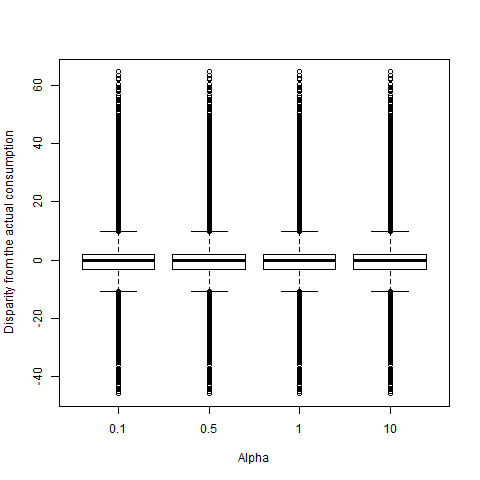
\includegraphics[scale=\figurescaling]{figures/db3/lrralphavariats.png}
	\caption{Electric power consumption dataset - Linear Ridge Regression with
	different $\alpha$ values}
	\label{ypmsd:fig:db3:lrrresults}
\end{figure}

\subsection{Nearest Neighbor}

Again following the method of applying $k-$nearest neighbors to previous two
datasets, three different variations of $k-$nearest neighbors with
$k\in\{2, 5, 10\}$ are selected to be applied against current dataset. Detailed
results are depicted in Table~\ref{ypmsd:table:ds3knnresults}.\\
Furthermore, distribution of prediction results with different $k$ are
demonstrated in Figure~\ref{ypmsd:fig:db3:nnrresults}.\\
According to these results, choosing $k$ as 2 has the lowest standard deviation
among all three. Meanwhile, choosing $k$ as 10 leads to a slighly better mean.

\begin{table}[p]
	\begin{center}
		\begin{tabular}{|c|c|c|c|}
			\hline	\backslashbox{$k$}{}&mean&standard deviaton&runtime(s)\\
\hline$2$&$0.028743182$&$3.887776774$&$05.975$\\
\hline$5$&$0.023519013$&$3.89919616$&$05.795$\\
\hline$10$&$0.011564662$&$4.064746421$&$05.782$\\\hline
\end{tabular}
\end{center}
\caption{Electric power consumption dataset - $k-$Nearest Neighbors}
\label{ypmsd:table:ds3knnresults}
\end{table}

\begin{figure}[p]
	\center
	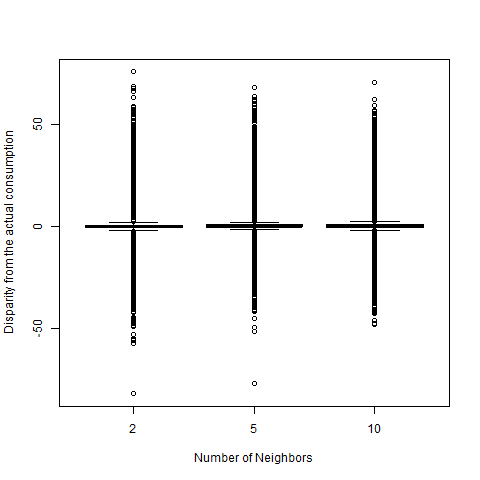
\includegraphics[scale=\figurescaling]{figures/db3/NNR.png}
	\caption{Electric power consumption dataset - Nearest Neighbor}
	\label{ypmsd:fig:db3:nnrresults}
\end{figure}

\subsection{Support Vector Machine}

As described in section \ref{ds2:svm}, support vector machine suffers a time
difficulty in bulding a model for large datasets. As a result, this method is skipped in
this section. Hence, no result is shown regarding applying support vector
machine on current dataset.

\subsection{Statistic Gradient Descent}

Applying statistics gradient descent with two different loss functions, {\it
squared\_loss} and {\it huber}, each one with two variant having $\epsilon \in
\{0.1, 1000\}$ results what is depicted in
Table~\ref{ypmsd:table:ds3sgdresults}. What is interesting is observing superior
outcome with smaller $\epsilon$ for {\it squared\_loss}. What's more, as it is
noticable, {\it squared\_loss} needs more time for building its model. Figure \ref{ypmsd:fig:db3:sgdresults} demonstrates distribution of differences between
predictions and actual data.



\begin{table}[p]
	\begin{center}
		\begin{tabular}{|c|c|c|c|c|}
			\hline	\backslashbox{$\epsilon$}{}&loss function&mean&standard
			deviaton&runtime(s)\\
\hline$0.1$&huber&$0.803895389$&$3.887776774$&$04.388$\\
\hline$0.1$&squared\_loss&$0.028169405$&$3.89919616$&$05.018$\\
\hline$1000$&huber&$0.105459652$&$4.064746421$&$04.411$\\
\hline$1000$&squared\_loss&$0.105459652$&$4.064746421$&$05.320$\\\hline
\end{tabular}
\end{center}
\caption{Electric power consumption dataset - Statistic Gradient Descent}
\label{ypmsd:table:ds3sgdresults}
\end{table}

\begin{figure}[p]
	\center
	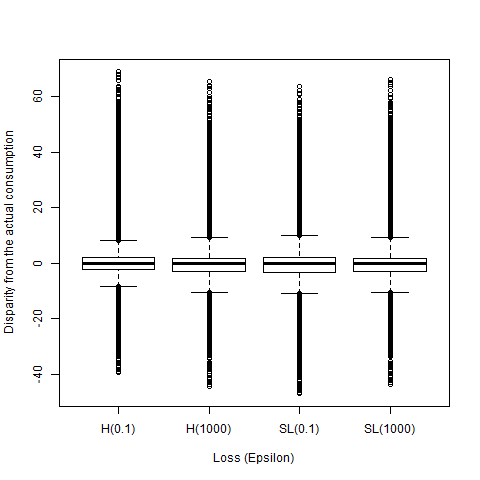
\includegraphics[scale=\figurescaling]{figures/db3/SGD.png}
	\caption{Electric power consumption dataset - Statistic Gradient Descent}
	\label{ypmsd:fig:db3:sgdresults}
\end{figure}


\subsection{Normalisation}
It was mentioned before that there wa an idea floating around to normalise
and scale Epoch numbers used rather than date .Most impacts are
expected to happen to algorithms which rely on distances between instances such
as $k-$Nearest Neighbors. Surprisingly not only it didn't
improve any result, but also caused models to make more mistakes and to provide
worse results.

\subsection{Comparison}
